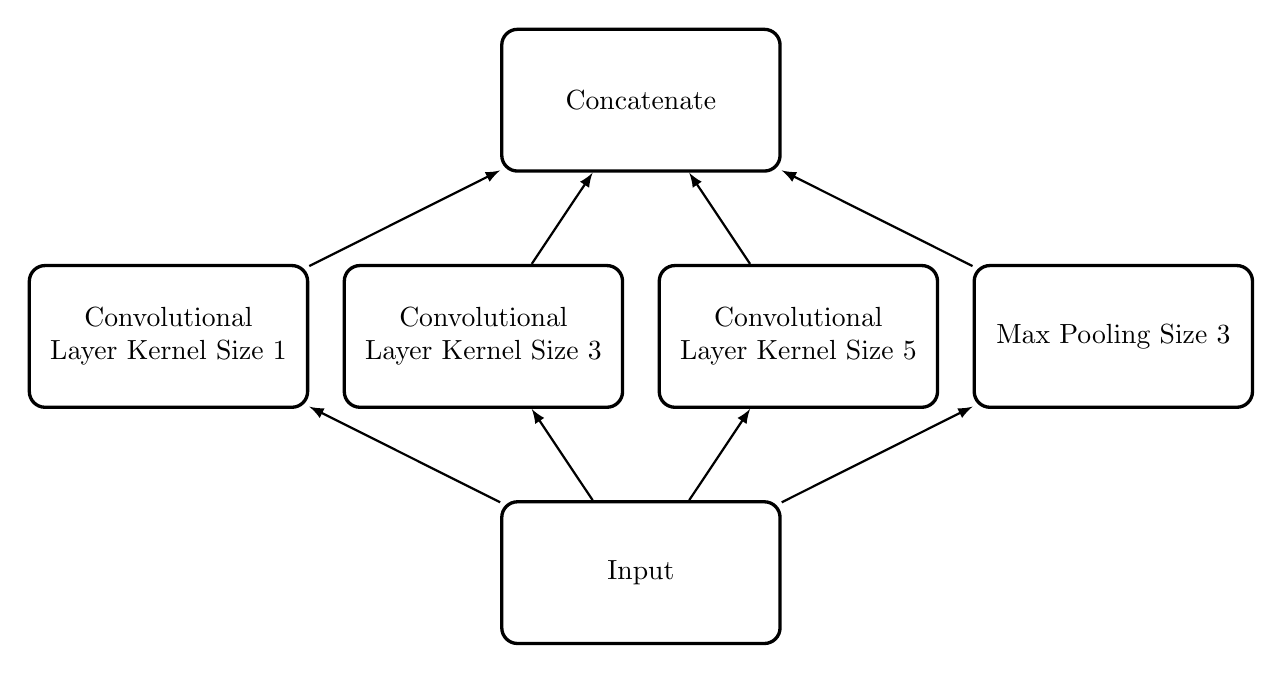
\begin{tikzpicture}[
	cell/.style={
		rectangle, 
		rounded corners=2mm, 
		draw,
		very thick,
		align=center,
		text width=3.3cm,
		minimum height=1.8cm
	},
	ArrowC1/.style={% Arrows with rounded corners
		rounded corners=.25cm,
		thick,
	},
]
	\node [cell] (out) at (0,6) {Concatenate};

	\node [cell] (c1) at (-6,3) {Convolutional Layer Kernel Size $1$};
	\node [cell] (c3) at (-2,3) {Convolutional Layer Kernel Size $3$};
	\node [cell] (c5) at (2,3) {Convolutional Layer Kernel Size $5$};
	\node [cell] (p) at (6,3) {Max Pooling Size $3$};
	
	\node [cell] (in) at (0,0) {Input};
	
	\draw [-latex,ArrowC1] (in) -- (c1);
	\draw [-latex,ArrowC1] (in) -- (c3);
	\draw [-latex,ArrowC1] (in) -- (c5);
	\draw [-latex,ArrowC1] (in) -- (p);
	\draw [-latex,ArrowC1] (c1) -- (out);
	\draw [-latex,ArrowC1] (c3) -- (out);
	\draw [-latex,ArrowC1] (c5) -- (out);
	\draw [-latex,ArrowC1] (p) -- (out);
\end{tikzpicture}